\section{Introduction}
Patient-specific computational models and simulations of the heart have increasingly  
been used to develop and guide clinical therapies~\cite{solis-lemus2023_reproducibility},
supporting the  
design~\cite{gray-2018-models_design,vanderlaan-2024-models_design}, 
evaluation~\cite{niederer-2019-models_evaluation,sung-2024-models_evaluation}, 
and delivery~\cite{lee-2018-models_delivery,dokuchaev-2023-models_delivery}
of innovative clinical therapies.
These models could advance personalised medicine by enabling the development and 
in-silico testing of therapies tailored to the anatomical and physiological features of individual patients.
However, the creation of credible and trustworthy cardiac models remains 
challenging~\cite{pras2018-intro-regulatory,jaffery-2024-review}.

There is growing support for the use of simulations for regulatory submission by the 
Medicines and Healthcare products Regulatory Agency~\cite{shepard-2015-mhra}, 
European Medicines Agency~\cite{ema2025_web}, and 
U.S. Food and Drug Administration (FDA)~\cite{jaffery-2024-review,fda2023_web}.
In particular, the FDA has identified scientific gaps and challenges that have limited 
the credibility of simulation models intended for medical use, including
(i) insufficient analytic methods, 
(ii) lack of established credibility assessment tools, 
(iii) absence of best-practice guidelines, and 
(iv) limited availability of high-quality, comprehensive data sets~\cite{fda2023_web}.

Data scarcity remains a fundamental obstacle to the development of robust cardiac models,
particularly the lack of high-quality, sex-balanced, disease-specific patient data. 
Several studies have attempted to bridge this gap through the creation of virtual cohorts that can 
be used for in-silico trials~\cite{strocchi2020_cohort,rodero2021_linking}.
Despite these advances, addressing sex balance in cardiac modeling databases is a persisting challenge. 

The cohort presented by Strocchi et al.~\cite{strocchi2020_cohort} has one 
female patient, while the one presented by Rodero et al.~\cite{rodero2021_linking} 
has 6 out of 20. Finally, in the study by Roney et al.~\cite{Roney2022-predicting} 
on predicting atrial fibrillation recurrence, 28 of the 99 patients were female.
Large virtual heart cohorts have begun to emerge, enabling in-silico trials and population-level 
analyses~\cite{passini2021_virtual,rodero-2021-virtualcohort1000,rodero-2021-virtualcohortextreme}. 
For example, the Strocchi et al.~\cite{strocchi2020_cohort} database has been 
widely used for studies on valve mechanics~\cite{feng2024_db_user}, 
fibrosis detection~\cite{okenov2024_db_user}, and 
arrhythmia modeling~\cite{kaboudian2023_db_user}.

While these cohorts represent valuable tools for the cardiac modelling community, 
they also highlight the challenge of having balanced representation of sex or disease subtypes, and 
workflows for generating new whole-heart cohorts remain poorly defined.

Sex bias is a complex, multi-factorial problem that affects the availability and generalisability 
of data used for computational models and simulations~\cite{steuernagel2023_sex_bias}.
Simulation studies can take considerable time and computational resources, 
which makes it especially relevant to consider whether anatomical differences associated with sex 
or disease influence the results.
The impact of such variation on simulation outcomes as well as on cardiac function is not frequently explored
or understood.
Understanding this relationship is key to determining when sex-specific anatomical data should be 
included in model development and evaluation.

Testing the importance of anatomical variability requires creating sex balanced virtual cohorts. 
However, building a model of the whole heart is a labour-intensive and technically demanding task.
Available solutions involve multiple stages: 
image segmentation, mesh generation, and the assignment of fibre orientations. 
Some approaches have explored the use of deep learning to automate aspects of 
mesh generation~\cite{pak2024_ai_meshes}. 
However, these methods are typically limited to single cardiac chambers rather than 
full four-chamber models.

CemrgApp~\cite{Razeghi2020-cemrgapp} is an open-source medical imaging platform with 
image processing toolkits for cardiovascular research, that has a low barrier to entry 
and low learning curve, putting reproducibility and best practices at the forefront.
CemrgApp has enabled semi-automated creation of high-quality left atrial models and 
has been employed in studies involving 
atrial fibrosis characterisation~\cite{Sim2019-reproducibility}, 
motion quantification~\cite{sillett2024_motion}, and 
regional strain analysis~\cite{sillett2023_strain1}. 
However, the extension of such tools to comprehensive whole-heart modelling, including 
all four chambers, has not been systematically demonstrated or standardised.

In this study, we developed CEMRG Heartbuilder, a Python-based library designed to systematically 
generate patient-specific, four-chamber heart models from clinical computerised tomography (CT) data. 
We applied the workflow to a new cohort of 50 patients (balanced by sex), 
classified into three clinical groups: controls ($n=26$), heart failure with narrow QRS ($n=12$), 
and heart failure with wide QRS ($n=12$). For each case, models were created from a CT scan 
to a simulation-ready mesh with fibres, and subsequently used to run benchmark electrophysiological and 
mechanical simulations. 
The simulations demonstrated the feasibility and robustness of the approach,
and, through the use of uniform material properties, isolated the impact of disease and sex differences 
in anatomy on reference mechanical and electro physiological simulations.

\replaced[id=PLOS, comment={PLOS: Fig (no period)}]{Fig}{Figure}~\ref{fig:heartbuilder_pipeline} 
provides an overview of the pipeline and the resulting cohort.

\begin{figure}[hbpt]
    \centering
    % File renamed from pics/fig1_graphical_abstract.pdf to pics/fig1_pipeline_overview.pdf
    % per EM round 2: this is the methods pipeline overview figure, not a graphical abstract.
    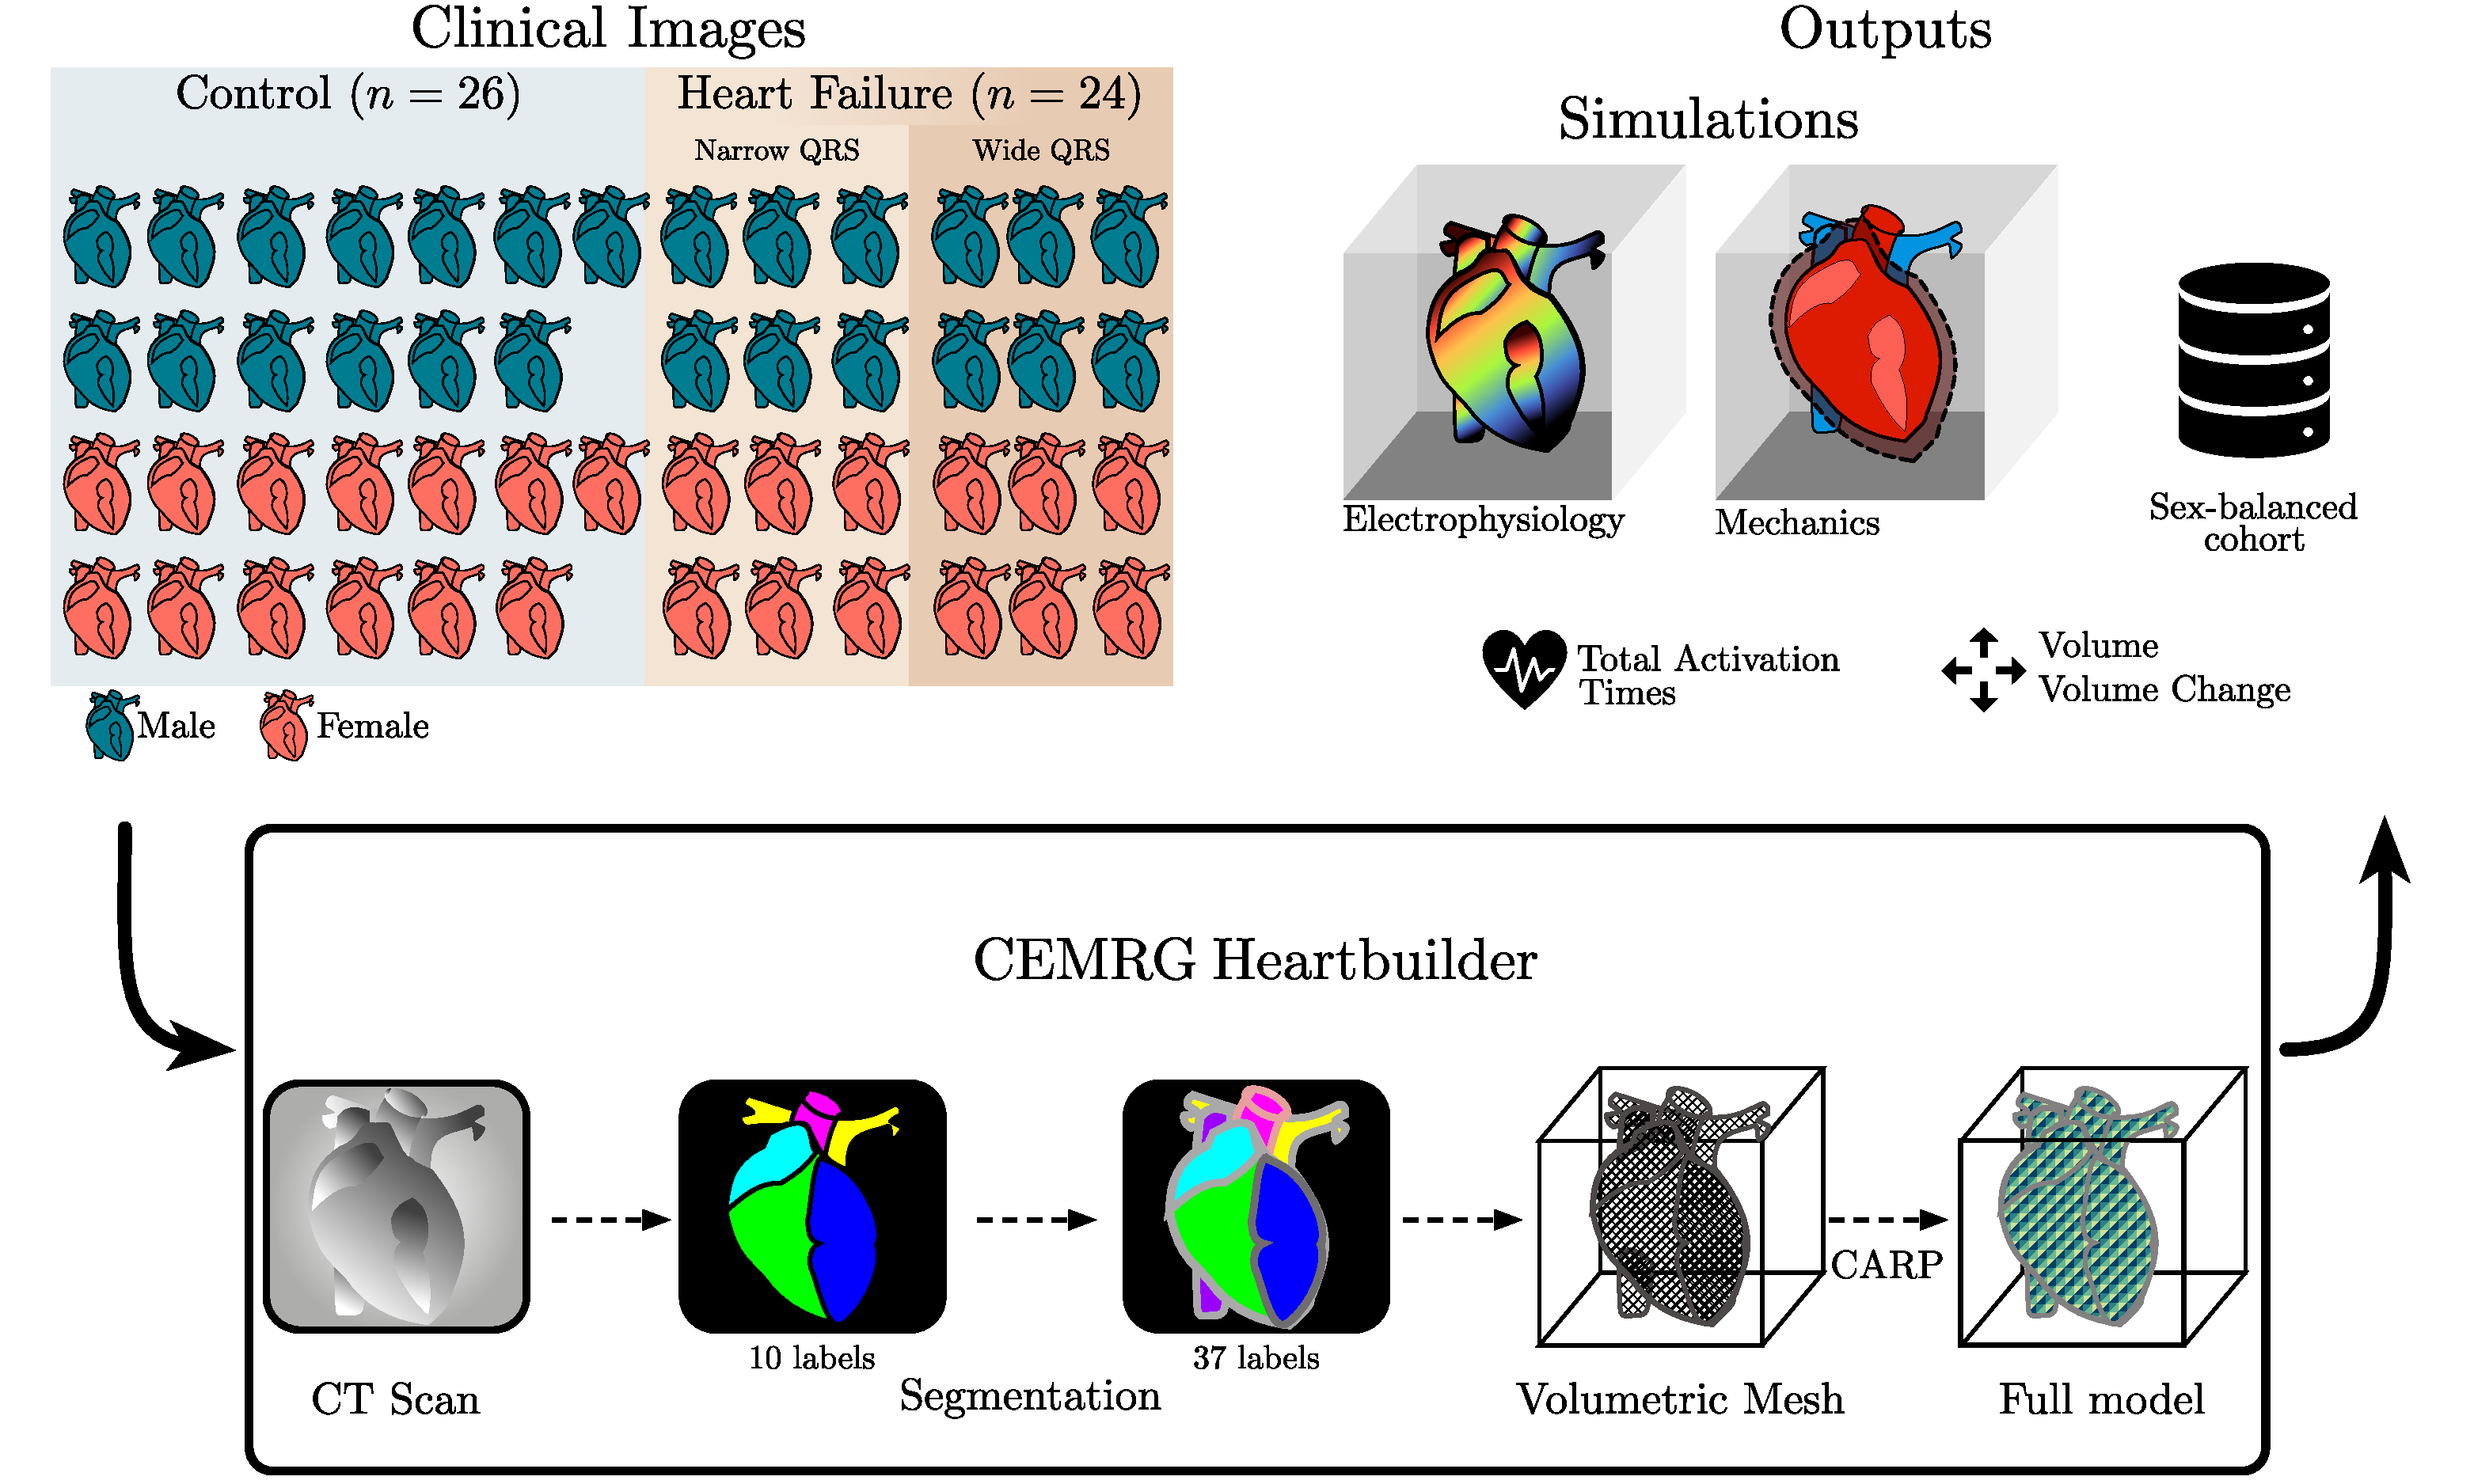
\includegraphics[width=\textwidth]{pics/fig1_pipeline_overview.pdf}
    \caption[Cohort creation and pipeline overview.]{
        \textbf{Cohort creation and pipeline overview. }
        Starting from clinical CT scans, the workflow performs multi-label segmentation and mesh generation
        to create simulation-ready models with assigned fibre orientations.
        A new dataset of 50 patients (26 controls, 24 with heart failure subtypes: narrow QRS and wide QRS)
        balanced by sex is processed.
        Resulting models are used in simulations of cardiac electrophysiology and mechanics to extract
        clinically relevant measurements.
        \added[id=PLOS, comment={EM: CC0 attribution for heart icons (already reported)}]{Heart icons in this figure were derived from a CC0 image obtained from openclipart.org (\url{https://openclipart.org/246884}) and modified to fit the figure design.}
    }
    \label{fig:heartbuilder_pipeline}
\end{figure}


% Thus, the objective is to create and a new cohort of 50 patient-specific, whole-heart models, 
% which include balanced representation of sex and classification into three clinical groups: 
% healthy controls, heart failure with narrow QRS, and heart failure with wide QRS.
% To generate these models in a reproducible and systematic way, we developed the CEMRG Heartbuilder pipeline, 
% a Python-based tool integrating custom image analysis routines with existing platforms
% to produce high-quality, simulation-ready meshes.
